\documentclass[11pt, letterpaper]{report}
\input{../../homework.tex}
\usepackage{titlepageBU}
\title{Honors Differential Equations}
\date{11/01/24}
\courseID{MA 231}
\professor{Dr. Wayne}
\courseSection{A1}
\DeclareMathOperator{\Tr}{Tr}
\begin{document}
\makeproblem
I've taken linear algebra before so I didn't show a ton of work when computing determinants and such, hopefully that's okay.

PLOT X(T) AND Y(T) FOR 3.5 PROBS 5,8
\section*{Section 3.2 Problem 1}
(a)
\[
	\lambda^2-\Tr (A)\lambda +\det (A)=\lambda ^2-\lambda -6=0\implies \lambda \in\left\{ -2,3 \right\} 
.\]
(b)
\[
	\begin{bmatrix} 3&2 \\ 0&-2 \end{bmatrix} \begin{bmatrix} x \\ y \end{bmatrix} =\begin{bmatrix} -2x \\ -2y \end{bmatrix} \implies \begin{bmatrix} 3x+2y \\ -2y \end{bmatrix} =\begin{bmatrix} -2x \\ -2y \end{bmatrix} \implies y=y
.\]
Fix $y=1$. Then $3x+2=-2x\implies x=-2 / 5$. We have $\lambda_{-}=-2$ and $\mathbf{v}_{-}=(-2 / 5,1)$.
\[
	\begin{bmatrix} 3&2 \\ 0&-2 \end{bmatrix} \begin{bmatrix} x \\ y \end{bmatrix} =\begin{bmatrix} 3x \\ 3y \end{bmatrix} \implies \begin{bmatrix} 3x+2y \\ -2y \end{bmatrix} =\begin{bmatrix} 3x \\ 3y \end{bmatrix} \implies 2y=0
.\]
Since $y=0$ and $x\in\mathbb{R}$ can be arbitrary, fix $x=1$. We then have $\lambda _{+}=3$ and $\mathbf{v}_{+}=(1,0)$.\\
(d)
\[
	\mathbf{Y}^{(-)}(t)=e^{-2t}\begin{bmatrix} -\frac{2}{5} \\ 1 \end{bmatrix} 
.\]
\begin{figure}[ht]
	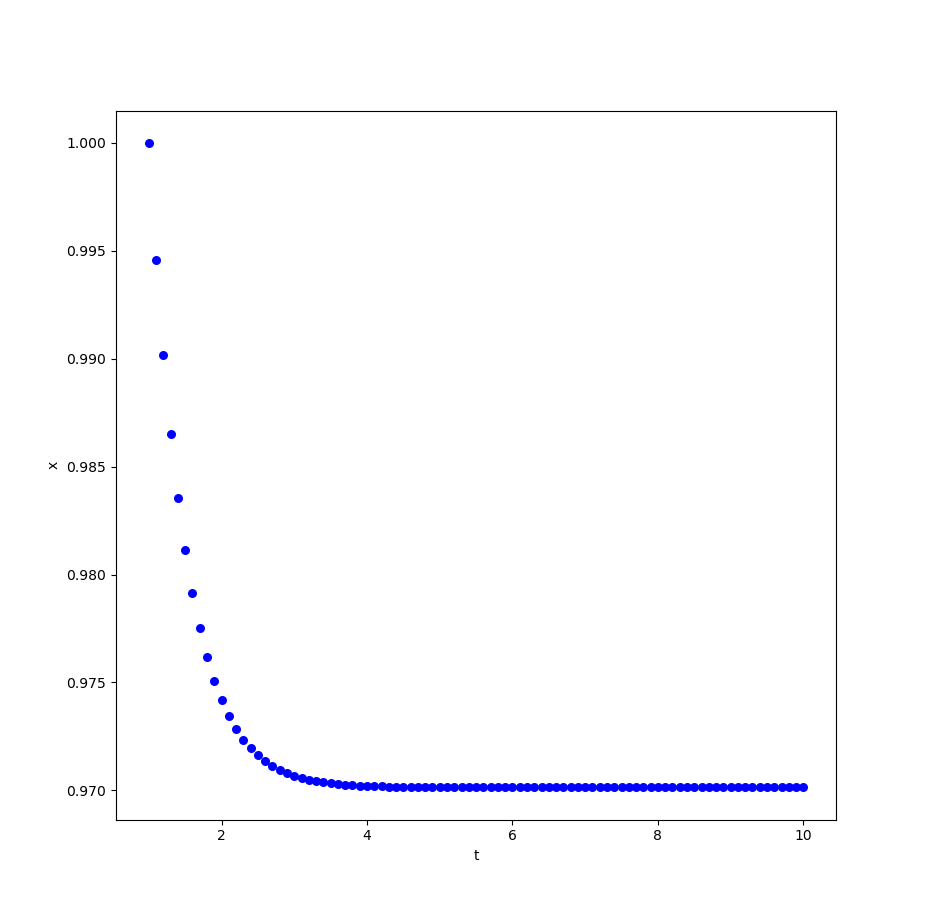
\includegraphics[scale=0.3]{3.2.1X.png}
	\centering
	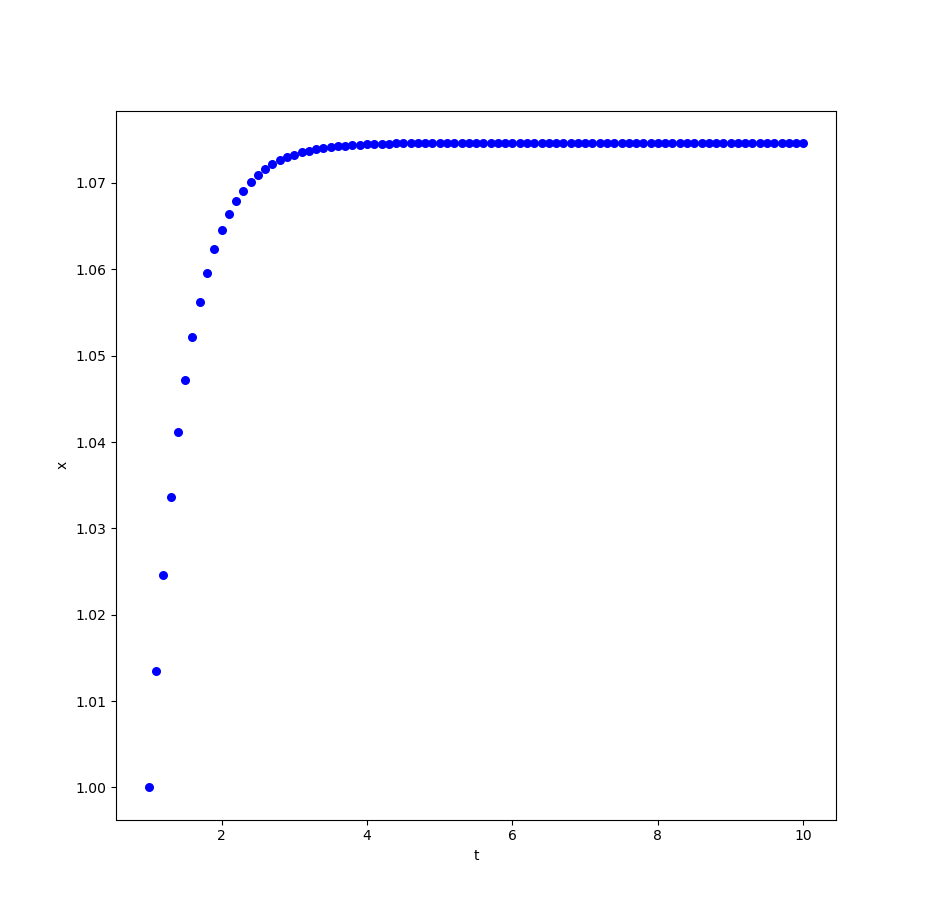
\includegraphics[scale=0.3]{3.2.1Y.png}
	\centering
\end{figure}
\[
	\mathbf{Y}^{(+)}(t)=e^{3t}\begin{bmatrix} 1 \\ 0 \end{bmatrix} 
.\]
Since $y(t)$ is constant and $0$, I have omitted it.
\begin{figure}[ht]
	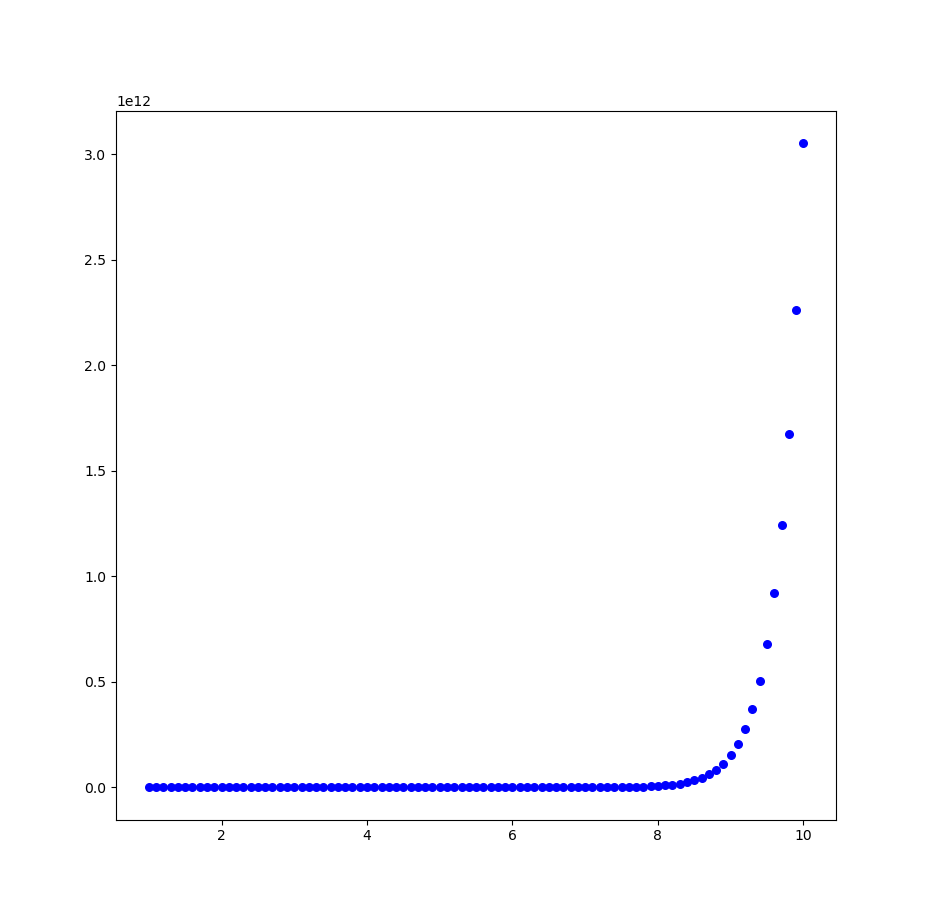
\includegraphics[scale=0.3]{3.2.1X2.png}
	\centering
\end{figure}

(e)
\[
	\mathbf{Y}(t)=c_1 \mathbf{Y}^{(-)}(t)+c_2 \mathbf{Y}^{(+)}(t)
.\]

\section*{Section 3.2 Problem 7}
(a)
\[
	\lambda ^2-\Tr (A)+\det (A)=\lambda ^2-3\lambda -4\implies \lambda \in \left\{ -1,4 \right\} 
.\]
(b)
\[
	\begin{bmatrix} 3&4 \\ 1&0 \end{bmatrix} \begin{bmatrix} x \\ y \end{bmatrix} =\begin{bmatrix} -x \\ -y \end{bmatrix} \implies \begin{bmatrix} 3x+4y \\ x \end{bmatrix} =\begin{bmatrix} -x \\ -y \end{bmatrix} \implies x=-y
.\]
Fix $x=1$. Then $y=-1$. We have $\lambda _{-}=-1$ and $\mathbf{v}_{-}=(1,-1)$.
\[
	\begin{bmatrix} 3x+4y \\ x \end{bmatrix} =\begin{bmatrix} 4x \\ 4y \end{bmatrix} \implies x=4y
.\]
Fix $y=1$. Then $x=4$. We then have $\lambda_{+}=4$ and $\mathbf{v}_{+}=(4,1)$.\\
(d)
\[
	\mathbf{Y}^{(-)}(t)=e^{-t}\begin{bmatrix} 1 \\ -1 \end{bmatrix} 
.\]
\begin{figure}[ht]
	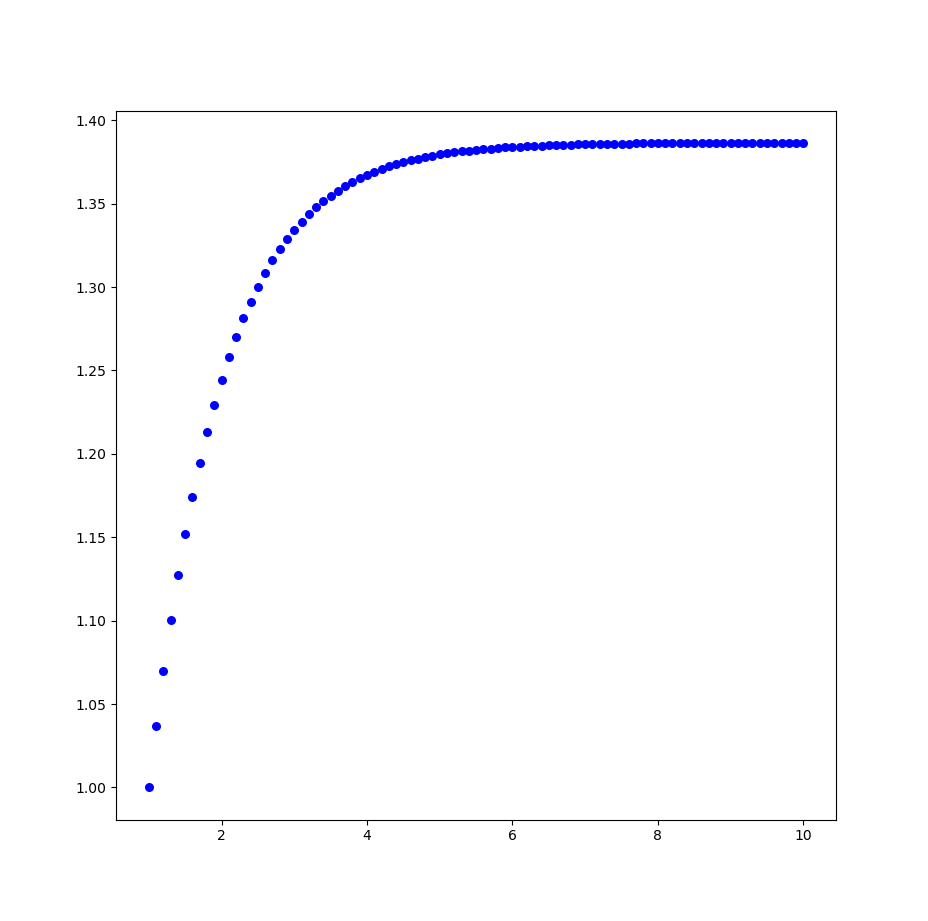
\includegraphics[scale=0.3]{3.2.1X1.png}
	\centering
	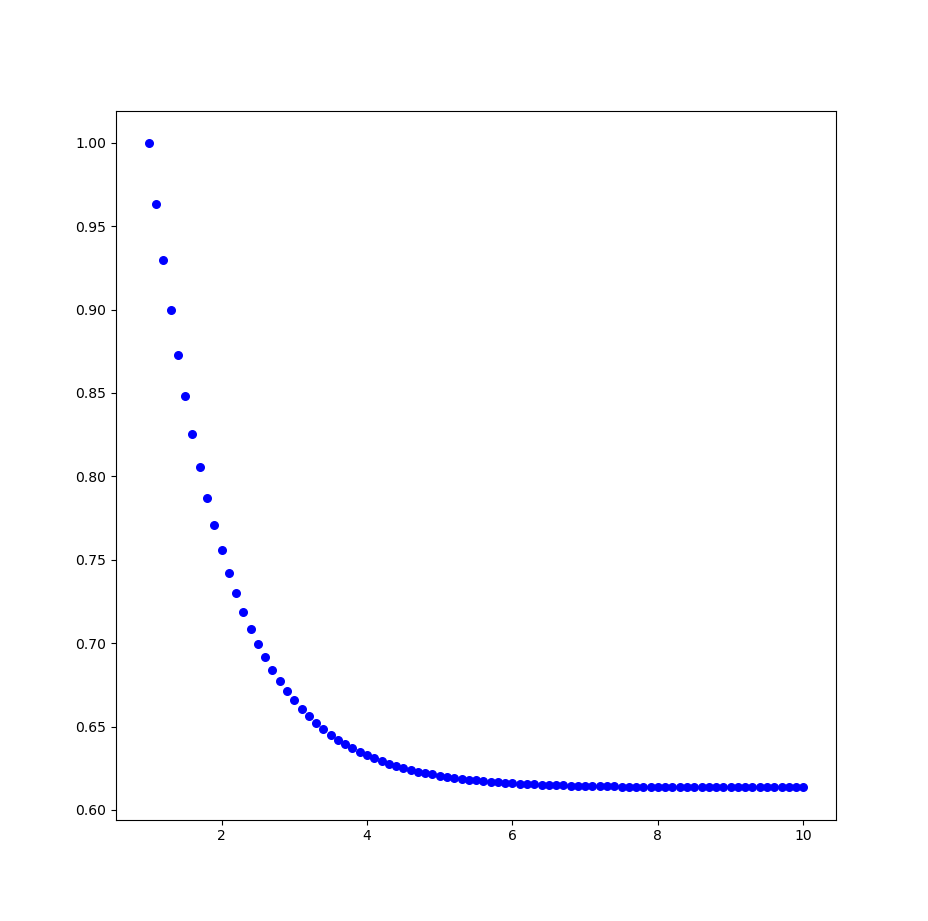
\includegraphics[scale=0.3]{3.2.2Y1.png}
	\centering
\end{figure}
\newpage
\[
	\mathbf{Y}^{(+)}(t)=e^{4t}\begin{bmatrix} 4 \\ 1 \end{bmatrix} 
.\]
\begin{figure}[ht]
	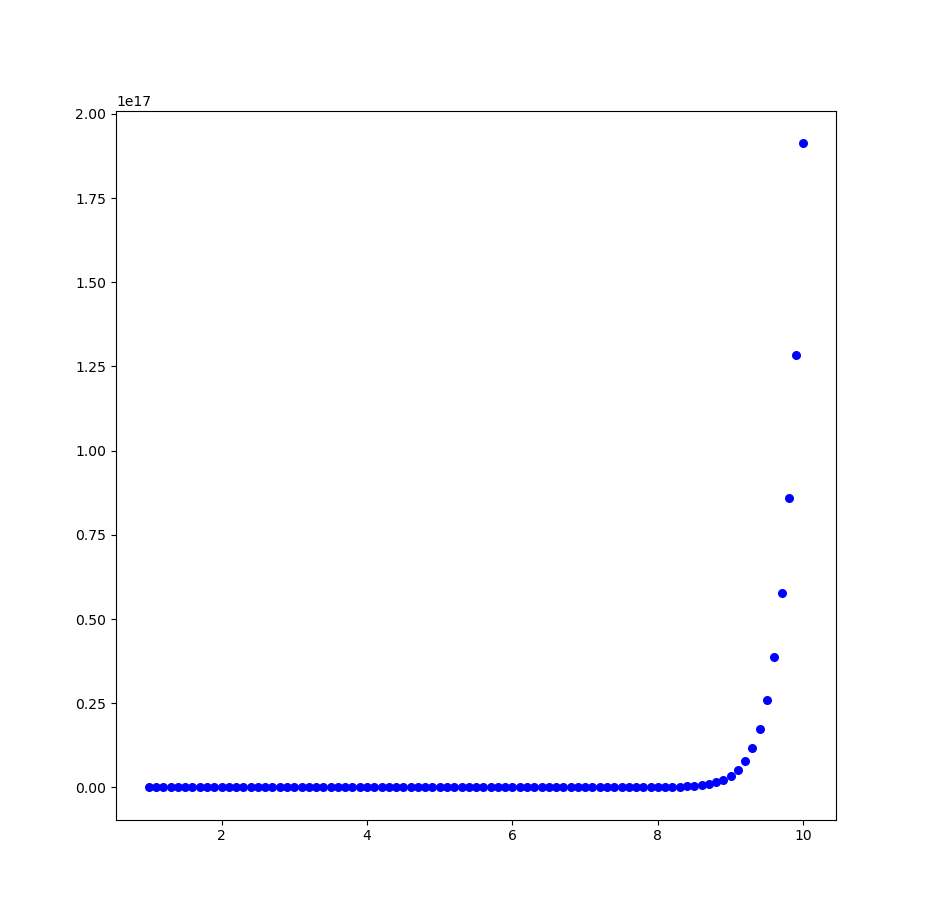
\includegraphics[scale=0.3]{3.2.2X2.png}
	\centering
	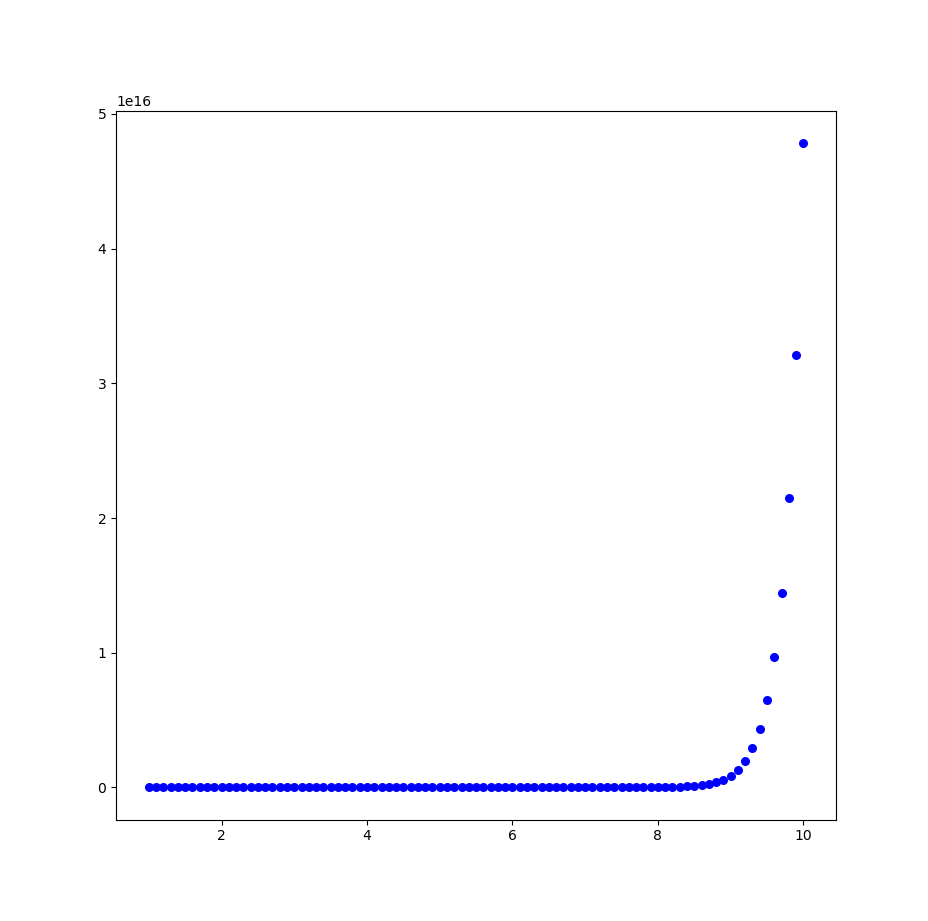
\includegraphics[scale=0.3]{3.2.2Y2.png}
	\centering
\end{figure}

(e)
\[
	\mathbf{Y}(t)=c_1 \mathbf{Y}^{(-)}(t)+c_2 \mathbf{Y}^{(+)}(t)
.\]
\section*{Section 3.2 Problem 18}
\[
	\lambda ^2-\Tr (A)\lambda +\det (A)=\lambda ^2-a\lambda -cb=0
.\]
\[
	\implies \lambda =\frac{a\pm \sqrt{a^2+4cb} }{2}
.\]
\section*{Section 3.2 Problem 19}
(a) Let $\frac{\mathrm{d}y}{\mathrm{d}t} =v$. Then
\[
	\frac{\mathrm{d}y}{\mathrm{d}t} =v,\qquad \frac{\mathrm{d}v}{\mathrm{d}t} +pv+qy=0
.\]
In matrix form,
\[
	\frac{\mathrm{d}\mathbf{Y}}{\mathrm{d}t} =\begin{bmatrix} 0&1 \\ -q&-p \end{bmatrix} \mathbf{Y}
,\]
where
\[
	\mathbf{Y}=\begin{bmatrix} y \\ v \end{bmatrix} 
.\]
(b)
\[
	\lambda ^2-\Tr (A)\lambda +\det (A)=\lambda ^2+p\lambda +q=0
.\]
(c)
\[
	\lambda ^2 + p\lambda +q=0\implies \lambda =\frac{-p\pm \sqrt{p^2-4q} }{2}	
.\]
(d) The eigenvalues are distinct for the discriminant nonzero, and are real for the discriminant nonnegative. Thus, we want $p^2-4q\in\mathbb{R}^+$.\\
(e) I actually don't see why the eigenvalues must be negative. Let $p^2-4q>0$, meaning the eigenvalues are real, but let $q=-p^2$. It follows that $p^2-4q=p^2+4p^2=5p^2$. Then
\[
	\frac{-p\pm \sqrt{5p^2} }{2}=\frac{-p\pm p\sqrt{5} }{2}
.\]
Since $\sqrt{5} >1$, this value should be positive for one of the solutions, no matter the sign of $p$.
\section*{Section 3.4 Problem 4}
\[
	\lambda ^2-8\lambda +20=0\implies \lambda =\frac{8\pm \sqrt{64-80} }{2}=4\pm 2i
.\]
Since $4>0$, the origin is a spiral source. The natural period is $\frac{2\pi}{2}=\pi $. Conversely, the natural frequency is $\frac{1}{\pi }$.
\[
	\begin{bmatrix} 2&2 \\ -4&6 \end{bmatrix} \begin{bmatrix} -1 \\ 1 \end{bmatrix} =\begin{bmatrix} 0 \\ 10 \end{bmatrix} 
.\]
Since we are to the left and above the origin on the phase plane, and the derivative vector is pointing straight up, we must be moving clockwise.
\begin{figure}[ht]
	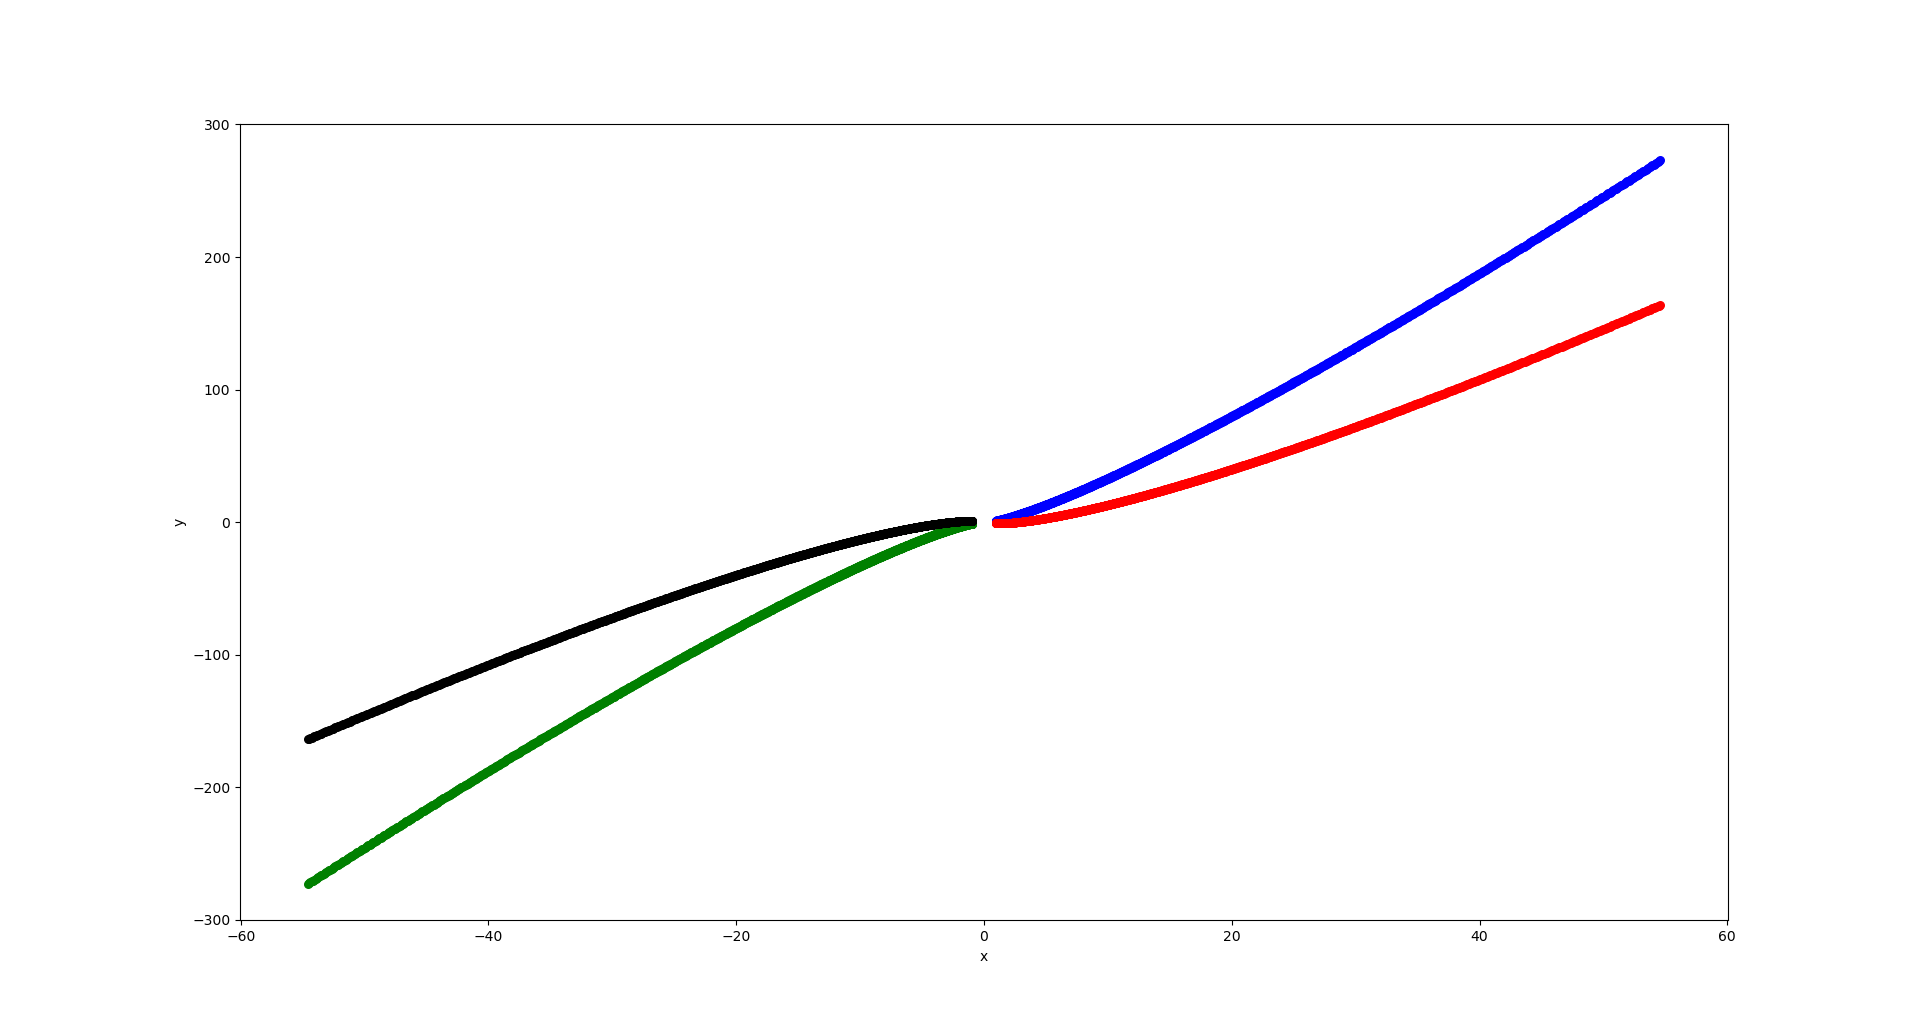
\includegraphics[scale=0.3]{3.4.5P.png}
	\centering
\end{figure}
\begin{figure}[ht]
	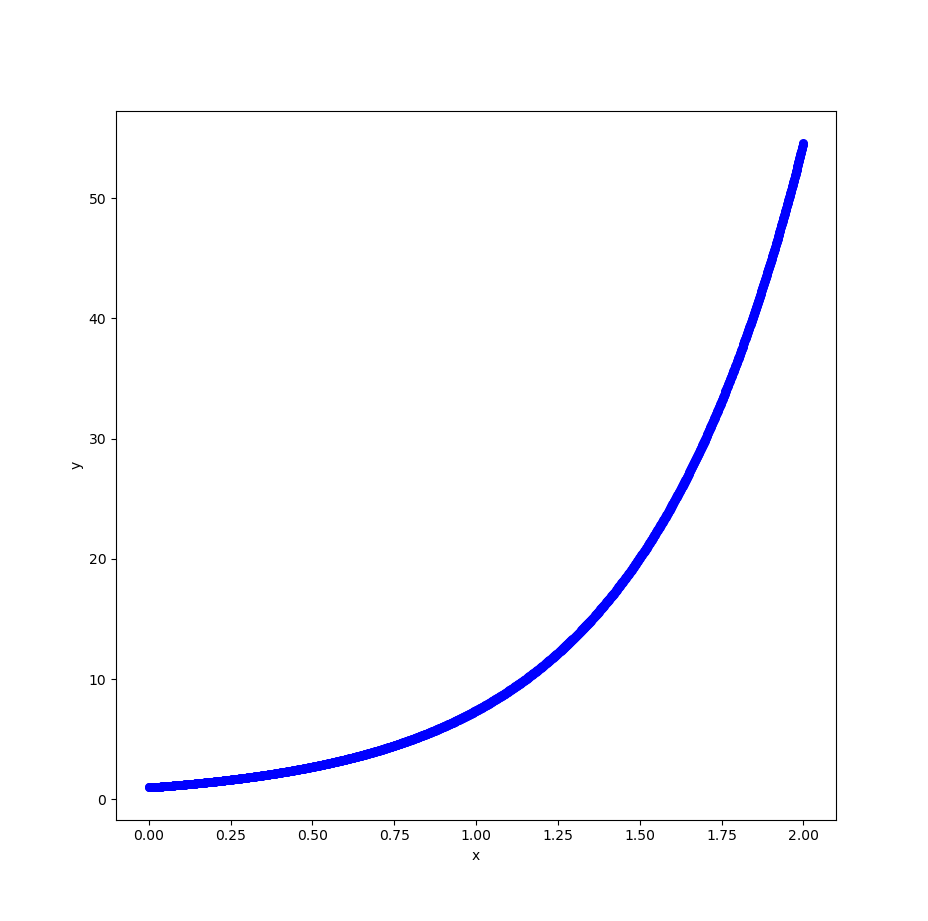
\includegraphics[scale=0.3]{3.4.5Y.png}
	\centering
	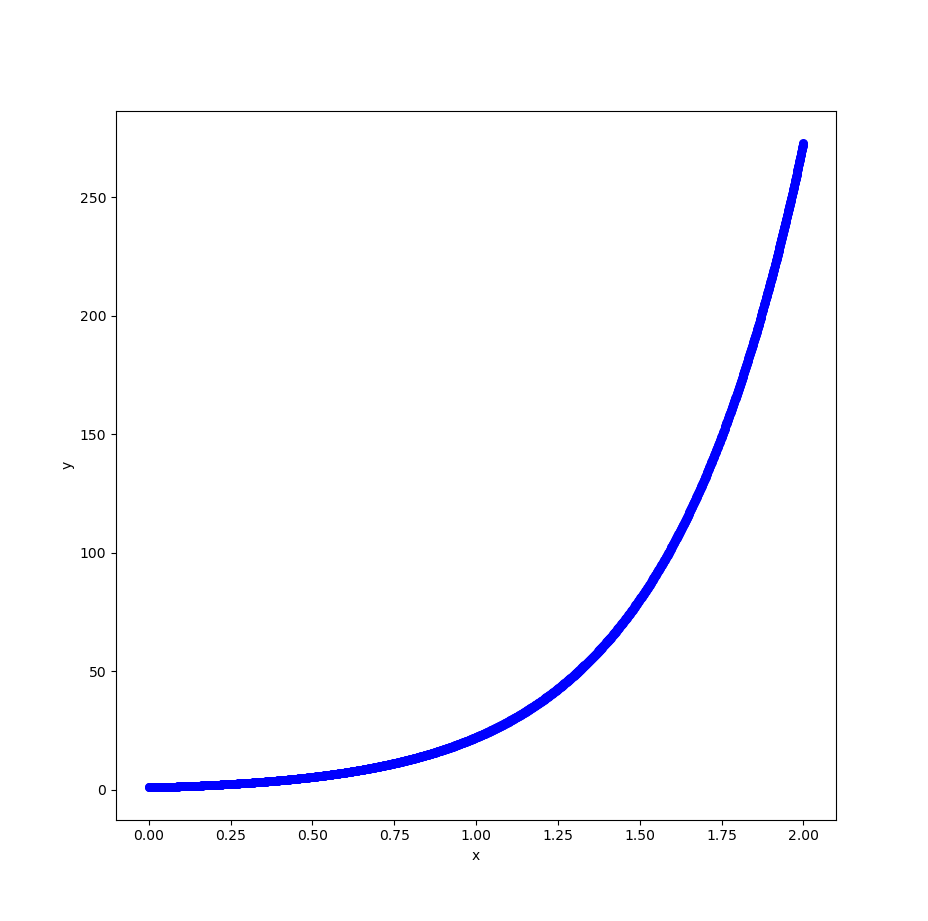
\includegraphics[scale=0.3]{3.4.5X.png}
	\centering
\end{figure}
\newpage
\section*{Section 3.4 Problem 5}
\[
	\lambda ^2+2\lambda +12=0\implies \lambda =\frac{-2\pm \sqrt{4-48} }{2}=\frac{-2\pm \sqrt{-44} }{2}=-1\pm i\sqrt{11}
.\]
Since $-1<0$, the origin is a spiral sink. The natural period is $2\pi / \sqrt{11} $. The natural frequency is then $\sqrt{11} / 2\pi $.
\[
	\begin{bmatrix} -3&-5 \\ 3&1 \end{bmatrix} \begin{bmatrix} 4 \\ 0 \end{bmatrix} =\begin{bmatrix} -12 \\ 12 \end{bmatrix} 
.\]
Since we are along the positive $x$-axis and the derivative vector is pointing upwards, we must be rotating counter-clockwise.
\begin{figure}[ht]
	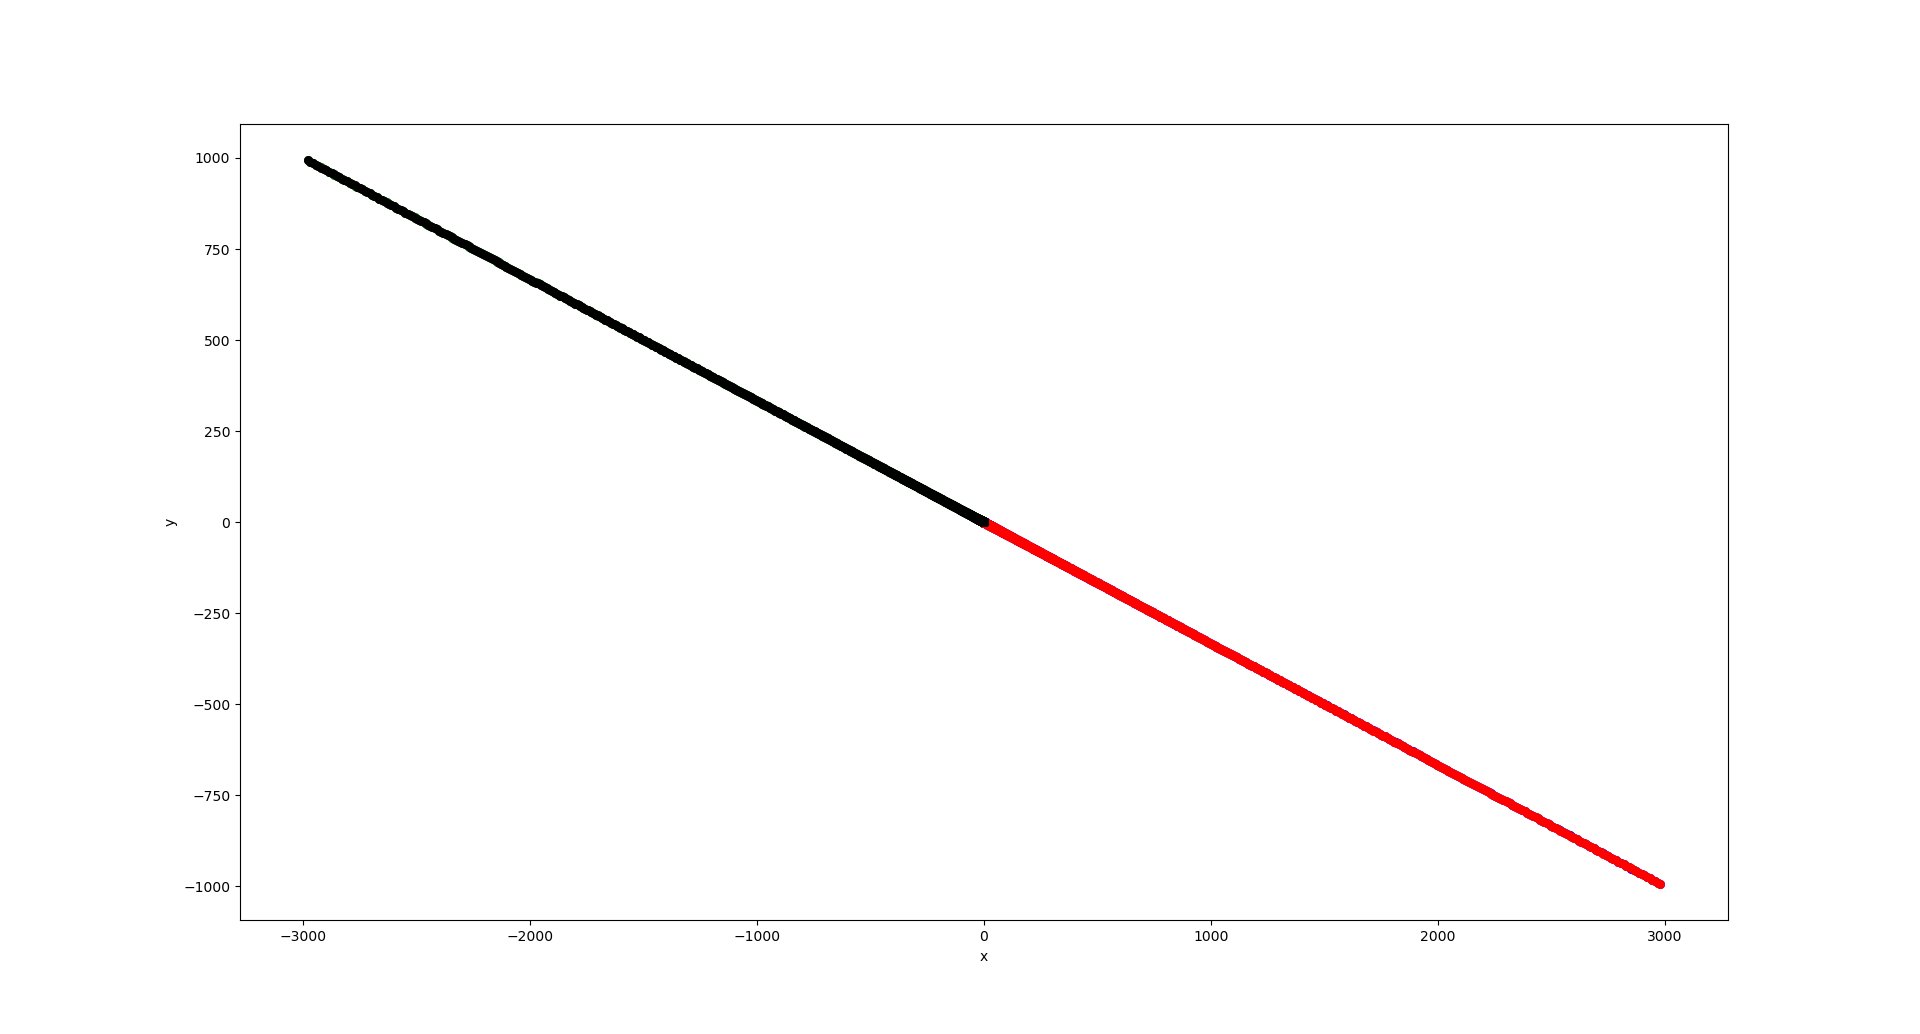
\includegraphics[scale=0.3]{3.4.6P.png}
	\centering
\end{figure}
\begin{figure}[ht]
	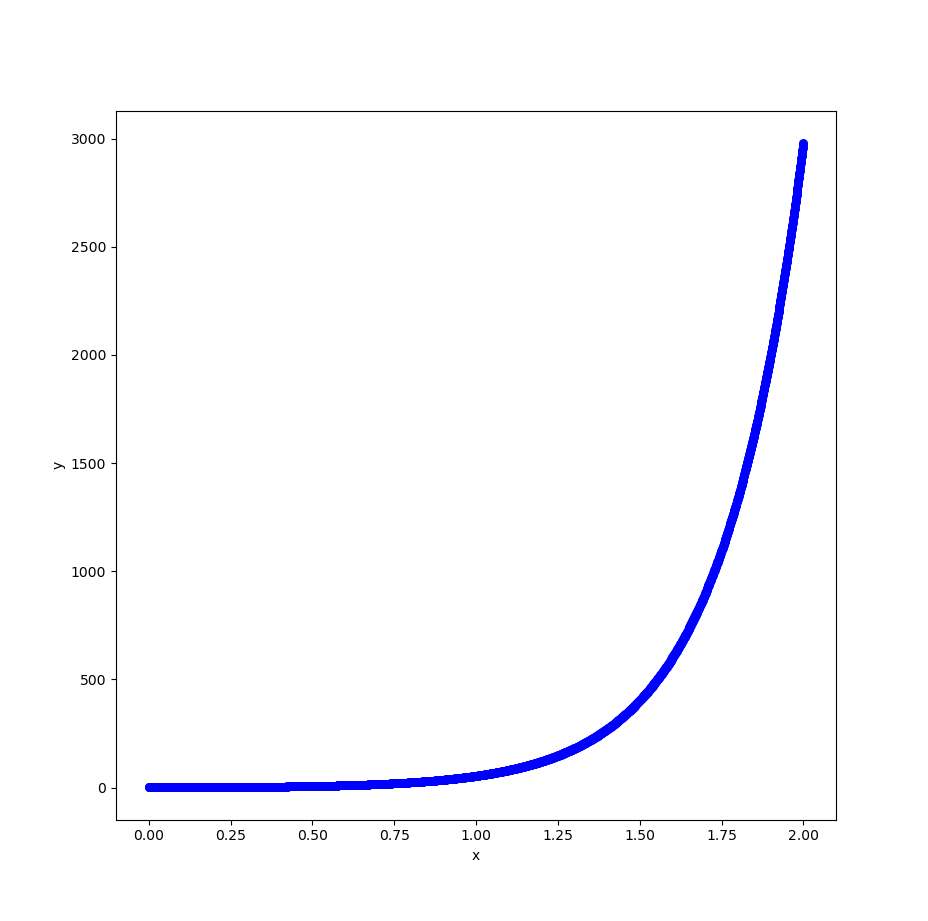
\includegraphics[scale=0.3]{3.4.6X.png}
	\centering
	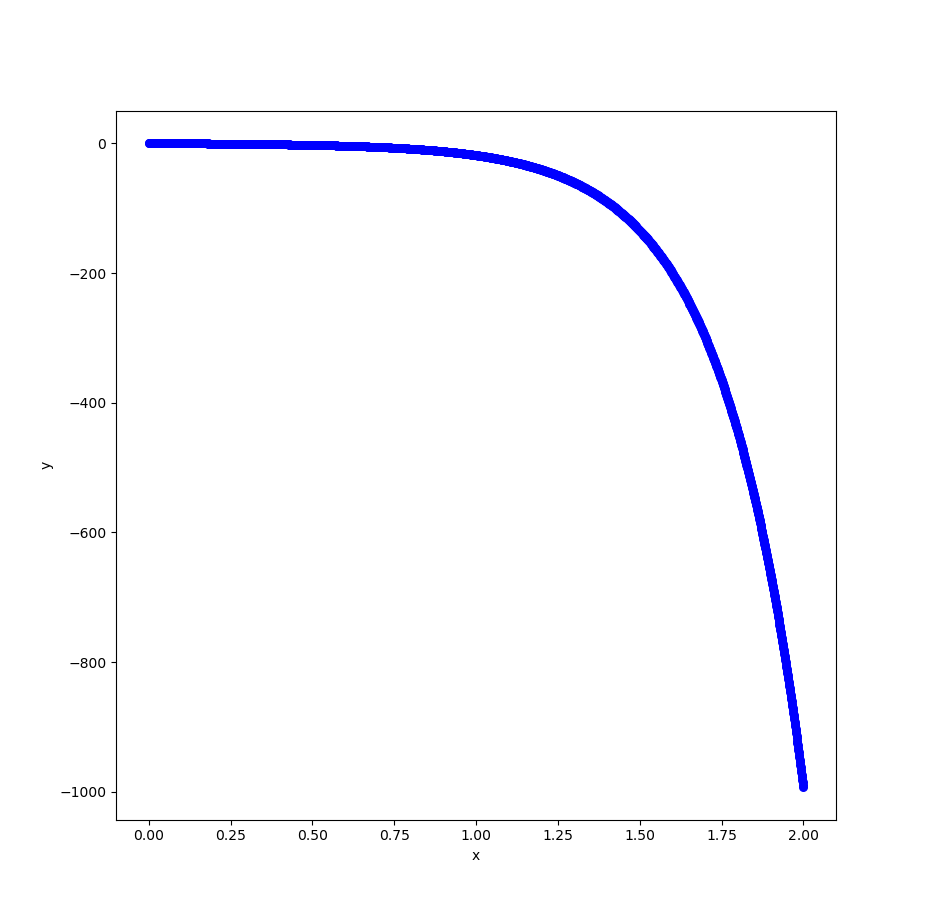
\includegraphics[scale=0.3]{3.4.6Y.png}
	\centering
\end{figure}
\section*{Section 3.4 Problem 15}
(i) cannot have complex eigenvalues, since its natural period changes with time. Since the natural period is the imaginary component of an eigenvalue which is constant, this cannot be the case for this system.\\
(ii) is a system with complex eigenvalues. The origin is a spiral sink and the natural frequency is approximately 3.\\
(iii) is not a system with complex eigenvalues, since the amplitude of the oscillations starts out large, then it goes through at least one entire period while being very small, then gets very large again. This means it is not exclusively approaching or diverging from the origin, and rather is doing different things at different times. Therefore, the origin is not a spiral sink or source, and the solution cannot have complex eigenvectors.\\
(iv) is a system with complex eigenvalues. The origin is a spiral sink and the natural frequency is approximately 1.5.\\
(v) is a system with complex eigenvalues. The origin is a spiral source and the natural frequency is approximately 3.\\
(vi) is a system with complex eigenvalues. The origin is a spiral source and the natural frequency is approximately 2.5.\\
\section*{Section 3.5 Problem 5}
\[
	\lambda ^2+6\lambda +9=0\implies \lambda =-3
.\]
\[
	\begin{bmatrix} -3&0 \\ 1&-3 \end{bmatrix} \begin{bmatrix} x \\ y \end{bmatrix} =\begin{bmatrix} -3x \\ -3y \end{bmatrix} \implies \begin{bmatrix} -3x \\ x-3y \end{bmatrix} =\begin{bmatrix} -3x \\ -3y \end{bmatrix} \implies x=0
.\]
Choose $y=1$. Then $\mathbf{v}=(0,1)$, and we have a solution
\[
	\mathbf{Y}_1(t)=c_1 e^{-3t}\begin{bmatrix} 0 \\ 1 \end{bmatrix} 
.\]
To find the other solution, notice that
\[
	\frac{\mathrm{d}x}{\mathrm{d}t} =-3x\implies x=e^{-3t}
.\]
Guess that $y=ate ^{kt}$. We have
\[
	\frac{\mathrm{d}y}{\mathrm{d}t} =akt e^{kt}+ae^{kt}=x-3y
.\]
Let $k=-3$ and $a=1$. Then
\[
	\frac{\mathrm{d}y}{\mathrm{d}t} =-3te^{-3t}+e^{-3t}=-3y+x
.\]
Therefore, we can make our second solution
\[
	\mathbf{Y}_2(t)=c_2 \begin{bmatrix} e^{-3t} \\ te ^{-3t} \end{bmatrix} 
.\]
The general solution is then
\[
	\mathbf{Y}(t)=c_1e^{-3t}\begin{bmatrix} 0 \\ 1 \end{bmatrix} +c_2 \begin{bmatrix} e^{-3t} \\ te ^{-3t} \end{bmatrix} 
.\]
Let $\mathbf{Y}(0)=(1,0)$. It follows that
\[
	c_1 \begin{bmatrix} 0 \\ 1 \end{bmatrix} +c_2 \begin{bmatrix} 1 \\ 0 \end{bmatrix} =\begin{bmatrix} 1 \\ 0 \end{bmatrix} 
.\]
Therefore, $c_1=1$ and $c_2=0$. Thus, the particular solution is
\[
	\mathbf{Y}_p(t)=e^{-3t}\begin{bmatrix} 0 \\ 1 \end{bmatrix} 
.\]
\begin{figure}[ht]
	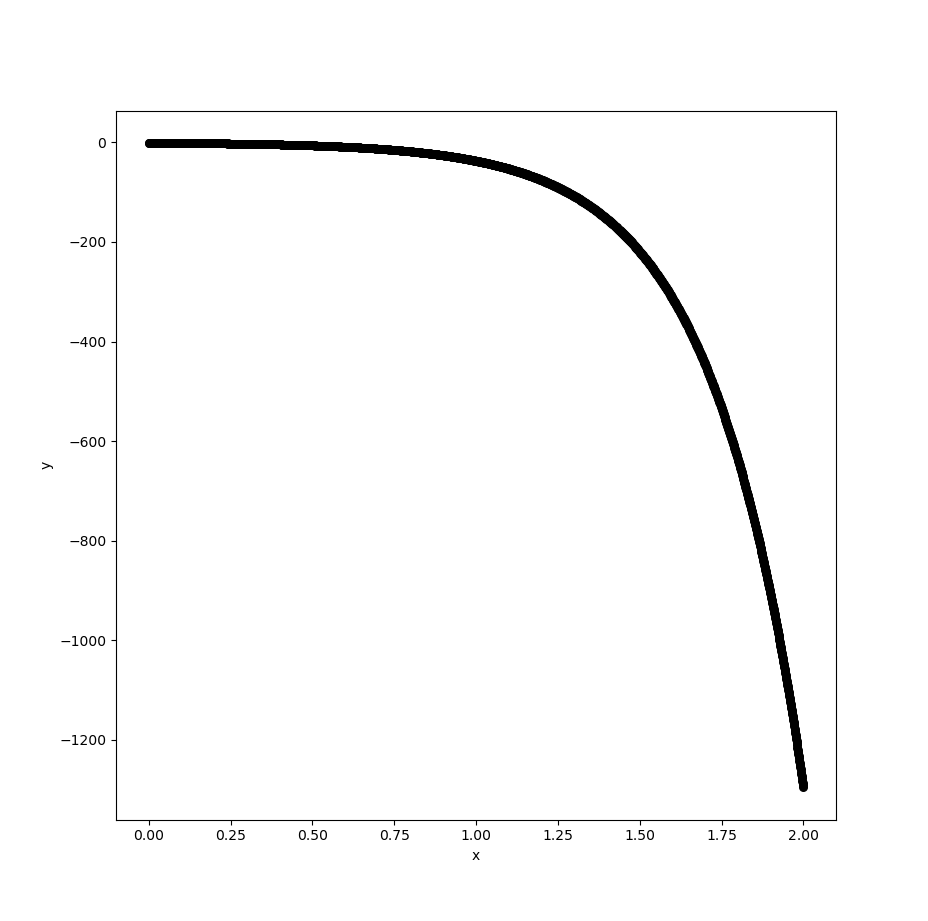
\includegraphics[scale=0.3]{3.5.5X.png}
	\centering
	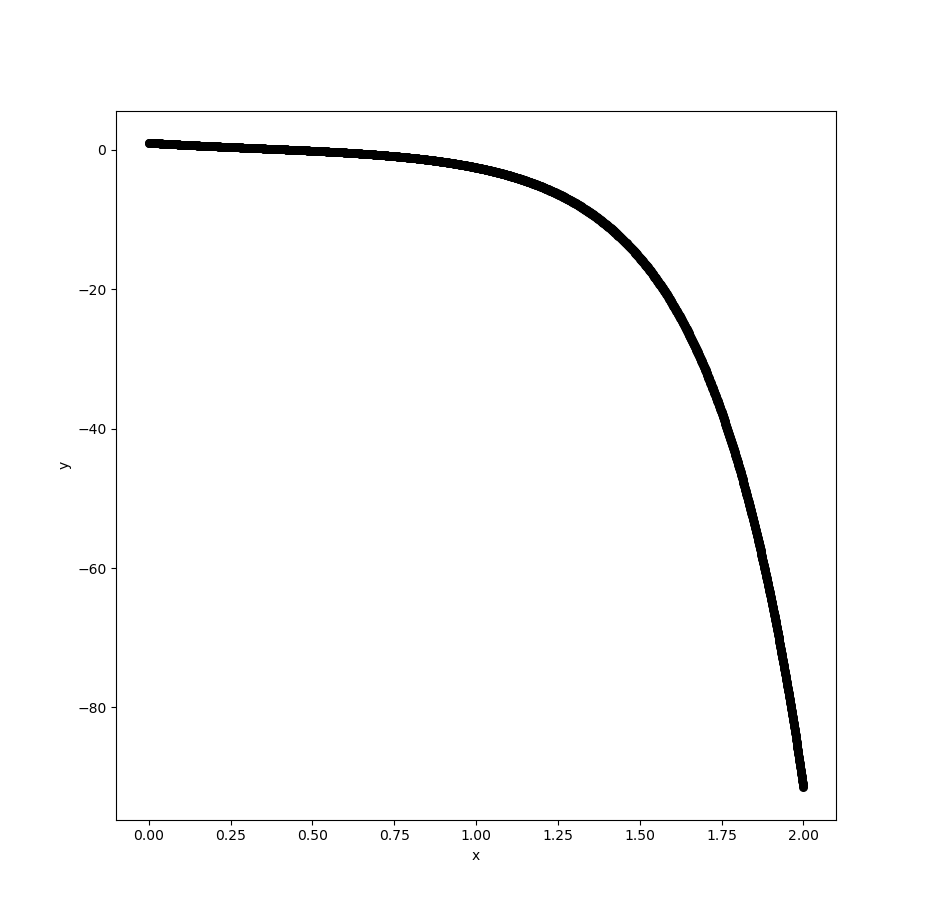
\includegraphics[scale=0.3]{3.5.5Y.png}
	\centering
\end{figure}
\section*{Section 3.5 Problem 8}
\[
	\lambda ^2+2\lambda +1=0 \implies \lambda=-1
.\]
\[
	\begin{bmatrix} 0&1 \\ -1&-2 \end{bmatrix} \begin{bmatrix} x \\ y \end{bmatrix} =\begin{bmatrix} -x \\ -y \end{bmatrix} \implies \begin{bmatrix} y \\ -x-2y \end{bmatrix} =\begin{bmatrix} -x \\ -y \end{bmatrix} \implies $y=-x$
.\]
Choose $x=1$. Then $\mathbf{v}=(1,-1)$, and our first solution is
\[
	\mathbf{Y}_1(t)=c_1 e^{-t}\begin{bmatrix} 1 \\ -1 \end{bmatrix} 
.\]
To find the other solution, guess that there exists a solution
\[
	\mathbf{Y}_2(t)=e^{-t}\left( t \mathbf{v}+\mathbf{w} \right)
.\]
It follows that
\[
	\frac{\mathrm{d}\mathbf{Y}_2}{\mathrm{d}t} =-e ^{-t}(t\mathbf{v}+\mathbf{w})+e^{-t}\mathbf{v}=e ^{-t}A\left( t\mathbf{v}+\mathbf{w} \right) 
.\]
Canceling the exponentials, we have
\[
	-t\mathbf{v}-\mathbf{w}+\mathbf{v}=tA\mathbf{v}+A\mathbf{w}
.\]
Since $-1$ is an eigenvalue, $-t \mathbf{v}=tA \mathbf{v}$, and we have
\[
	-\mathbf{w}+\mathbf{v}=A \mathbf{w}
.\]
Solving for $\mathbf{w}$, it follows that
\[
	\begin{bmatrix} 1-w_1 \\ -1-w_2 \end{bmatrix} =\begin{bmatrix} 0&1 \\ -1&-2 \end{bmatrix} \begin{bmatrix} w_1 \\ w_2 \end{bmatrix} =\begin{bmatrix} w_2 \\ -w_1-w_2 \end{bmatrix} 
.\]
From the bottom entries of the matrices, we have $-1-w_2=-w_1-w_2$. Cancelling the negative, we have $1+w_2=w_1+w_2$. It follows that $w_1=1$, and thus $w_2=0$ by the top component. Therefore, our second solution is
\[
	\mathbf{Y}_2(t)=c_2e^{-t}\begin{bmatrix} t+1 \\ t \end{bmatrix}
.\]
The general solution is thus
\[
	\mathbf{Y}(t)=c_1e^{-t}\begin{bmatrix} 1 \\ -1 \end{bmatrix} +c_2e^{-t}\begin{bmatrix} t+1 \\ t \end{bmatrix} 
.\]
Taking $\mathbf{Y}(0)=(1,0)$, we have
\[
	c_1 \begin{bmatrix} 1 \\ -1 \end{bmatrix} +c_2 \begin{bmatrix} 1 \\ 0 \end{bmatrix} =\begin{bmatrix} 1 \\ 0 \end{bmatrix} \implies \begin{bmatrix} c_1+c_2 \\ -c_1 \end{bmatrix} =\begin{bmatrix} 1 \\ 0 \end{bmatrix} 
.\]
It follows that $c_1=0$ and $c_2=1$. Therefore, our particular solution is
\[
	\mathbf{Y}_p(t)=e^{-t}\begin{bmatrix} t+1 \\ t \end{bmatrix} 
.\]
\begin{figure}[ht]
	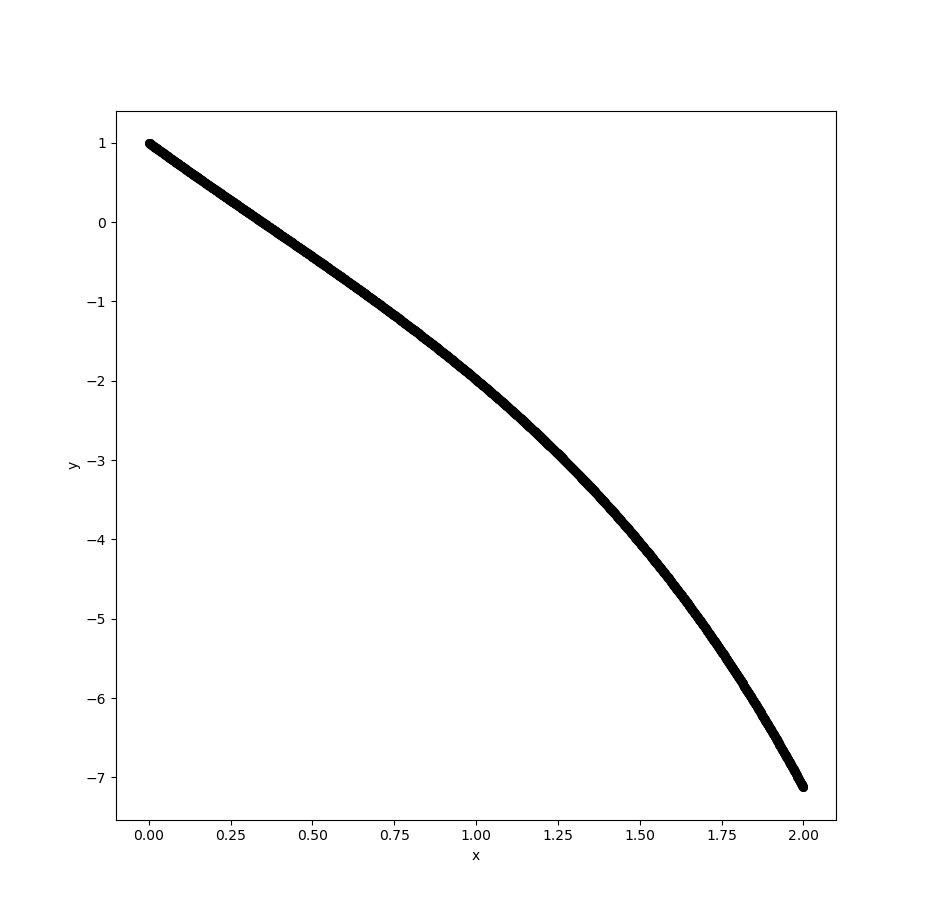
\includegraphics[scale=0.3]{3.5.8Y.png}
	\centering
	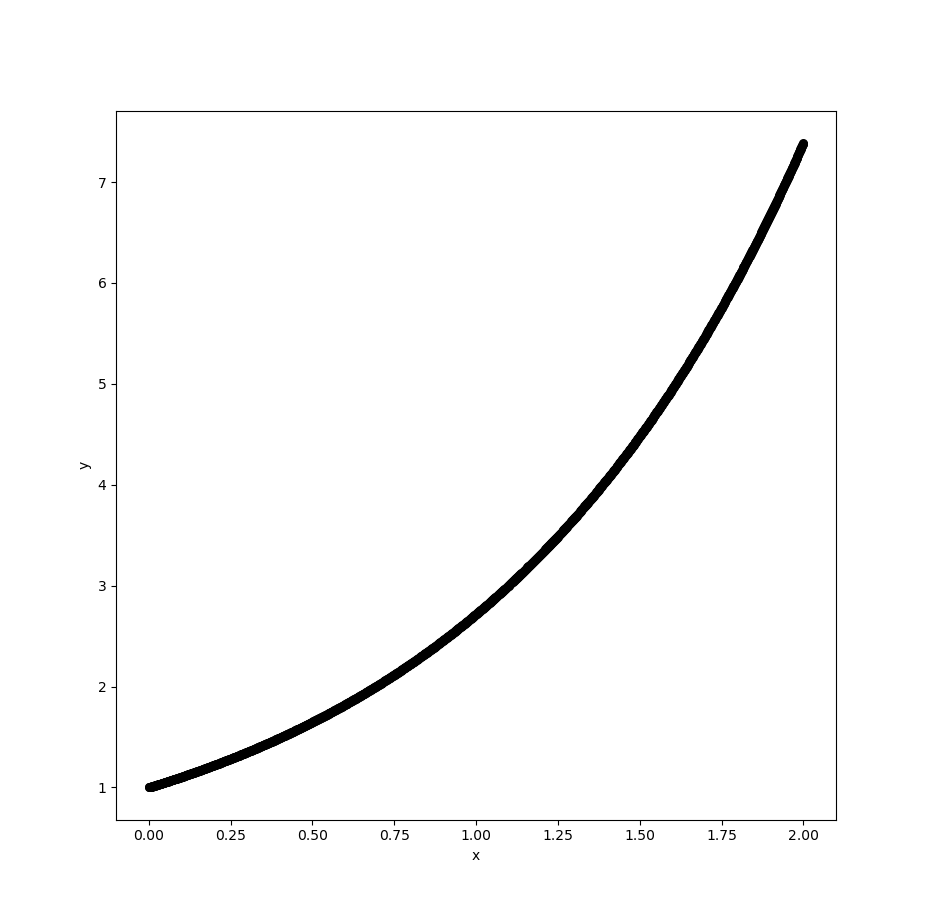
\includegraphics[scale=0.3]{3.5.8X.png}
	\centering
\end{figure}
\section*{Section 3.5 Problem 13}
Note that $(1,0),(0,1)\in\mathbb{R}^2$, and since the eigenspace corresponding to the eigenvalue $\lambda $ is $m\mathbb{R}^2$, we have $\mathbf{A}(1,0)=(\lambda ,0)$, and likewise for $(0,1)$. Note that
\[\begin{bmatrix} a&b \\ c&d \end{bmatrix} \begin{bmatrix} 1 \\ 0 \end{bmatrix} =\begin{bmatrix} a \\ c \end{bmatrix} =\begin{bmatrix} \lambda  \\ 0 \end{bmatrix} .\]
It follows that $c=0$ and $a=\lambda $. Furthermore, note that
\[
	\begin{bmatrix} a&b \\ c&d \end{bmatrix} \begin{bmatrix} 0 \\ 1 \end{bmatrix} =\begin{bmatrix} b\\ d \end{bmatrix} =\begin{bmatrix} 0 \\ \lambda  \end{bmatrix} 
.\]
Therefore, $b=0$ and $d=\lambda $. It follows that
\[
	\mathbf{A}=\begin{bmatrix} \lambda &0 \\ 0&\lambda  \end{bmatrix} =\operatorname{diag }(\lambda ,\lambda ) 
.\]
\section*{Section 3.5 Problem 14}
Since $\mathbf{Y}_1,\mathbf{Y}_2\in\mathbb{R}^2$ are linearly independent, and since $\dim \mathbb{R}^2=2$, then $\left\{ \mathbf{Y}_1,\mathbf{Y}_2 \right\} $ spans $\mathbb{R}^2$, and thus every vector $\mathbf{v}\in\mathbb{R}^2$ can be written as
\[
	\mathbf{v}=c_1 \mathbf{Y}_1+c_2\mathbf{Y}_2
\]
for some $c_1,c_2\in\mathbb{R}$. It follows that
\[
	\mathbf{Av}=\mathbf{A}\left( c_1 \mathbf{Y}_1+c_2 \mathbf{Y}_2 \right) =c_1 \mathbf{AY}_1+c_2 \mathbf{AY}_2=c_1\lambda \mathbf{Y}_1+c_2\lambda \mathbf{Y}_2=\lambda \left( c_1\mathbf{Y}_1 +c_2 \mathbf{Y}_2\right) =\lambda \mathbf{v}
.\]
Therefore, $\mathbf{Av}=\lambda \mathbf{v}$ for all $\mathbf{v}\in\mathbb{R}^2$.
\section*{Review 19}
I have listed the systems in order, from (i) to (viii). My analysis of which corresponds to which image comes after.
\begin{align*}
	\frac{\mathrm{d}x}{\mathrm{d}t} &=x+y,&\frac{\mathrm{d}y}{\mathrm{d}t} &=-2x-y\\
	\frac{\mathrm{d}x}{\mathrm{d}t} &=-3x+y,&\frac{\mathrm{d}y}{\mathrm{d}t} &=-x+y\\
	\frac{\mathrm{d}x}{\mathrm{d}t} &=-3x+y,&\frac{\mathrm{d}y}{\mathrm{d}t} &=-x\\
	\frac{\mathrm{d}x}{\mathrm{d}t} &=-x+y,&\frac{\mathrm{d}y}{\mathrm{d}t} &=-2x+y\\
	\frac{\mathrm{d}x}{\mathrm{d}t} &=2x,&\frac{\mathrm{d}y}{\mathrm{d}t} &=x-y\\
	\frac{\mathrm{d}x}{\mathrm{d}t} &=3x+y,&\frac{\mathrm{d}y}{\mathrm{d}t} &=-x\\
	\frac{\mathrm{d}x}{\mathrm{d}t} &=y,&\frac{\mathrm{d}y}{\mathrm{d}t} &=-4-4\\
	\frac{\mathrm{d}x}{\mathrm{d}t} &=-3x-3y,&\frac{\mathrm{d}y}{\mathrm{d}t} &=2x+y
.\end{align*}
From our knowledge of the trace-determinant plane, we know graph (a) must have $\Tr (A)=0$ and $\det (A)>0$. Only systems (i) and (iv) have  $\Tr (A)=0$, but they both have $\det A>0$. Notice however that for $x>0$ and $y<0$, system (i) can have a positive $\frac\mathrm{dx}{\mathrm{d}t} $, which it clearly shouldn't from the image. However, in the case of (iv), $\frac{\mathrm{d}x}{\mathrm{d}t} $ will always be negative, which matches the image. Therefore, (a) is (iv).

From our knowledge of the trace-determinant plane, we know graph (b) must have negative trace and
 \[
	\det A=\frac{1}{4}\left( \Tr A \right) ^2,\quad \Tr A<0
.\]
(ii), (iii), (vii), and (viii) have negative trace. Of those, only (vii) satisfies the above equation. Therefore, (b) is (vii).

From our knowledge of the trace-determinant plane, we know graph (c) must have negative determinant. Only (ii) and (v) satisfy this. Consider the point $(0,1)$. Graph (c) has positive x and y at this point. (ii) gives the vector $(1,1)$, which satisfies this, whereas (v) gives the vector $\left( 0,-1 \right) $, which clearly does not. Also note that (v) is triangular, and the eigenvalue $-1$ does not match the straight line solution we can see. Therefore, (c) is (ii).

From our knowledge of the trace-determinant plane, we know graph (d) must have positive trace and
 \[
	\det A=\frac{1}{4}\left( \Tr A \right) ^2
.\]
(iv), (v), and (vi) have positive trace, but we have already used (iv) and (v), so the solution is (vi).
\section*{Review 21}
I have listed the systems in order, from (i) to (viii). My analysis of which corresponds to which image comes after.
\begin{align*}
	\frac{\mathrm{d}x}{\mathrm{d}t} &=3x+4y&\frac{\mathrm{d}y}{\mathrm{d}t} &=x\\
	\frac{\mathrm{d}x}{\mathrm{d}t} &=2x&\frac{\mathrm{d}y}{\mathrm{d}t} &=x+5y\\
	\frac{\mathrm{d}x}{\mathrm{d}t} &=-3x-2y&\frac{\mathrm{d}y}{\mathrm{d}t} &=-y\\
	\frac{\mathrm{d}x}{\mathrm{d}t} &=-y&\frac{\mathrm{d}y}{\mathrm{d}t} &=4x\\
	\frac{\mathrm{d}x}{\mathrm{d}t} &=x+2y&\frac{\mathrm{d}y}{\mathrm{d}t} &=-5x-y\\
	\frac{\mathrm{d}x}{\mathrm{d}t} &=x+0.25y&\frac{\mathrm{d}y}{\mathrm{d}t} &=0.25x+y\\
	\frac{\mathrm{d}x}{\mathrm{d}t} &=-1.1x-2y&\frac{\mathrm{d}y}{\mathrm{d}t} &=2x-1.1y\\
	\frac{\mathrm{d}x}{\mathrm{d}t} &=-1.1x-5y&\frac{\mathrm{d}y}{\mathrm{d}t} &=x+0.9y
.\end{align*}
(a) has negative determinant, and since I'm doing (a) last, the only remaining option is (i). So (a) goes with (i).

(b) must have positive trace and determinant, with
\[
	\det A<\frac{1}{4}\left( \Tr A \right) ^2
.\]
This is only satisfied by (ii) and (vi). However, the equations are symmetric, and since (ii) is triangular, we can see its eigenvalues are not symmetric such that the graph would look like this. So (b) goes with (vi).

(c) must have a trace of 0, which only (iv) and (v) have. Notice that at $t=0$, the rate of change of one variable is temporarily 0, and the other is at a maximum. Additioanlly, $(x,y)\approx (1,0)$. Plugging this into (iv) produces the desired behavior, while (v) does not. So (c) goes with (iv).

(d) must have positive determinant, negative trace, and it must have
\[
	\det A>\frac{1}{4}\left( \Tr A \right) ^2
.\]
This is satisfied by (vii) and (viii). I noticed that in about one second, $x$ drops by 4, suggesting that it is the one with $-5$ in it, meaning (viii) satisfies graph (d).
\section*{Section 4.1 Problem 7}
First, we guess a particular solution of the form $ae^{4t}$. We have
\[
	\frac{\mathrm{d}y}{\mathrm{d}t} =4ae^{4t},\quad \frac{\mathrm{d}^2y}{\mathrm{d}t^2} =16ae^{4t}
.\]
It follows that
\[
	\frac{\mathrm{d}^2y}{\mathrm{d}t^2} -5 \frac{\mathrm{d}y}{\mathrm{d}t} +4y=16ae^{4t}-20ae^{4t}+4ae^{4t}=0
.\]
Since this didn't work, we guess a solution of the form $tae^{4t}$. We have
\[
	\frac{\mathrm{d}y}{\mathrm{d}t} =4tae^{4t}+ae^{4t},\quad \frac{\mathrm{d}^2y}{\mathrm{d}t^2} =16tae^{4t}+8ae^{4t}
.\]
It follows that
\[
	\frac{\mathrm{d}^2y}{\mathrm{d}t^2} -5 \frac{\mathrm{d}y}{\mathrm{d}t} +4y=16tae^{4t}+8ae^{4t}-20tae^{4t}-5ae^{4t}+4tae^{4t}=e^{4t}
.\]
Cancelling the exponents and combining like terms, we ahve
\[
	3a=1\implies a=\frac{1}{3}
.\]
Therefore,
\[
	y_p(t)=\frac{t}{3}e^{4t}
\]
is a particular solution to the equation.

Now consider the homogeneous case. Let $v=\frac{\mathrm{d}y}{\mathrm{d}t} $, and note that
\[
	\frac{\mathrm{d}\mathbf{Y}}{\mathrm{d}t} =\begin{bmatrix} 4&-5 \\ 0&1 \end{bmatrix} \mathbf{Y}
,\]
where $\mathbf{Y}=(v,y)$. Since this matrix is triangular, note that it has eigenvalues $1$ and $4$. Solving for eigenvectors, we have
\[
	\begin{bmatrix} 4&-5 \\ 0&1 \end{bmatrix} \begin{bmatrix} y \\ v \end{bmatrix} =\begin{bmatrix} y \\ v \end{bmatrix} \implies \begin{bmatrix} 4y-5v \\ v \end{bmatrix} =\begin{bmatrix} y \\ v \end{bmatrix} 
.\]
Notice that $3y=5v$. Fixing $v=3$, we have $y=5$. Therefore, $\lambda =1$ corresponds to $\mathbf{v}=(3,5)$.
\[
	\begin{bmatrix} 4&-5 \\ 0&1 \end{bmatrix} \begin{bmatrix} y \\ v \end{bmatrix} =\begin{bmatrix} 4y \\ 4v \end{bmatrix} \implies \begin{bmatrix} 4y-5v \\ v \end{bmatrix} =\begin{bmatrix} 4y \\ 4v \end{bmatrix} 
.\]
It follows that $v=0$. Let $y=1$. We then have $\lambda =4$ corresponding to the eigenvector $(0,1)$.

It follows that solutions to $y(t)$ are simply
\[
	y(t)=c_1e^{4t}+c_2e^{t}+\frac{t}{3}e^{4t}
.\]
Note here that I absorbed the 5 into the constant $c_2$, and left out the $v$s since we only care about $y(t)$.
\section*{Section 4.1 Problem 13}
First, we guess a particular solution of the form $ae^{-t/2}$. Notice that
\[
	\frac{\mathrm{d}y}{\mathrm{d}t} =-\frac{a}{2}e^{-t / 2},\quad \frac{\mathrm{d}^2y}{\mathrm{d}t^2} =\frac{a}{4}e^{-t /2}
.\]
It follows that
\[
	\frac{\mathrm{d}^2y}{\mathrm{d}t^2} +4 \frac{\mathrm{d}y}{\mathrm{d}t} +3y=\frac{a}{4}e^{-t /2}-2ae^{-t / 2}+3ae^{-t /2}=e^{-t /2}
.\]
Dividing out the exponentials, we have
\[
	\frac{a}{4}-2a+3a=1\implies \frac{5}{4}a=1\implies a=\frac{4}{5}
.\]
We then have a particular solution
\[
	y_p(t)=\frac{4}{5}e^{-t /2}
.\]
We now compute the general solution. Let $v=\frac{\mathrm{d}y}{\mathrm{d}t} $, and notice that
\[
	\frac{\mathrm{d}\mathbf{Y}}{\mathrm{d}t} =\begin{bmatrix} 3&4 \\ 0&1 \end{bmatrix} \begin{bmatrix} y \\ v \end{bmatrix} 
.\]
Since this matrix is triangular, it has eigenvalues 3 and 1. Solving for the eigenvectors, we have
\[
	\begin{bmatrix} 3y+4v \\ v \end{bmatrix} =\begin{bmatrix} y \\ v \end{bmatrix}
.\]
Choose $v=1$. We have $y=-2$, and $(-2,1)$ is our eigenvector for $\lambda =1$.
\[
	\begin{bmatrix} 3y+4v \\ v \end{bmatrix} =\begin{bmatrix} 3y \\ 3v \end{bmatrix} 
.\]
We have $v=0$ and $y=1$. Putting this together, we have the general solution
\[
	y(t)=c_1e^{3t}+c_2e^{t}+\frac{4}{5}e^{-t /2}
.\]
For $y(0)=y'(0)=0$, we have
\[
	\frac{\mathrm{d}^2y}{\mathrm{d}t^2} =1
.\]
It follows that
\[
	9c_1+c_2+\frac{1}{5}-\frac{2}{5}+\frac{4}{5}+c_2+3c_1+c_1+c_2=13c_1+12c_2+\frac{1}{5}=1
.\]
Thus,
\[
	13c_1+12c_2=\frac{4}{5}
.\]
Let $c_1=0$. Then $c_2=1 / 15$. We then have
\[
	y(t)=\frac{1}{15}e^{t}+\frac{4}{5}e^{-t /2}
.\]

The terms from the homogeneous solution will eventually overpower the term from the inhomogeneous solution due to the larger exponents, so as $t\to \infty$, $y\to \infty$ as well, unless the coefficients are negative in which case $y\to -\infty$.
\section*{Supplimental 1}
At the fixed point, $z_{n+1}=z_n$ for all $n$. Thus, let $r=2$ and let
\[
	z_n = rz_n(1-z_n)=2z_n-2z_n^2
.\]
It follows that
\[
	2z_n^2-z_n=0
.\]
\[
	z_n(2z_n-1)=0\implies z_n=\frac{1}{2}
.\]
Therefore, the fixed point is $\frac{1}{2}$. This aligns with our analysis in the previous homework.
\section*{Supplimental 2}
Let $p_1 = 3.2p_2(1-p_2)=3.2(p_2-p_2^2)$, and let $p_2=3.2p_1(1-p_1)=3.2(p_1-p_1^2)$. Plugging in, we have
\begin{align*}
	p_2&=3.2\left( 3.2\left( p_2-p_2^2 \right)  \right) \left( 1-3.2\left( p_2-p_2^2 \right)  \right)
.\end{align*}
Plugging into a calculator because no thanks, we have the following approximate solutions:
\[
	p_2\in \left\{ 0,0.513045,0.6875,0.799455 \right\} 
.\]
We will ignore $0$, and solve for $p_1$ given each of these values of $p_2$. For $p_2=0.513045$, $p_1=0.200545$ or $p_1=0.799455$, which is another possible value of $p_2$. Similarly, for $p_2=0.799455$, $p_1=0.513045$ or $p_1=0.48695$. For $p_2=0.6875$, $p_1=0.6875$ or $0.3125$. I assume this means $0,6875$ is a fixed point, and since $0.799455$ and $0.513045$ are the closest together pairs of points that correspond, they constrain the solution within them. This assumption lines up with the previous homework's numerics, but it's really confusing with all the 0s and I don't really know what's happening.
\section*{Supplimental 3}
The bifurcation is at $r=3$. I have no idea why.
\section*{Supplimental 4}
First, consider the base case $n=1$. It follows that $x^n-y^n=x-y$. Since $x-y=x-y$, $x-y$ divides $x-y$ trivially. Therefore, the base case holds. Additionally, note that
\[
	\frac{x-y}{x-y}=1
,\]
which is a $0$-th degree polynomial. Since $1-1=0$, the claim holds.

Now consider the inductive case. Suppose for some positive integer $n$ that $x^n-y^n$ is divisible by $x-y$, and that the resultant polynomial is of degree $n-1$. We wish to show that $x^{n+1}-y^{n+1}$ is divisible by $x-y$, and that the resultant polynomial is of degree $n$. Notice that
\[
	x^{n+1}-y^{n+1}=x^{n+1}-yx^{n}+yx^{n}-y^{n+1}=x^n(x-y)-y\left( x^n-y^n \right) 
.\]
By the inductive hypothesis, since $x-y$ divides $x^n-y^n$, there exists a polynomial $P$ such that $x^n-y^n=P(x-y)$. It follows hat
\[
	x^n(x-y)-y\left( x^n-y^n \right) =x^n(x-y)-y(x-y)P=(x-y)\left( x^n-yP \right) 
.\]
Clearly, $(x-y)$ divides this. Additionally, note that the order of the polynomial in $x$ is $n$, which is equal to $n+1-1$. Additionally, by the inductive hypothesis, $P$ has degree $n-1$ in $x$ and $y$, so $yP$ has degree $n$ in $y$. Therefore, our polynomial has degree $n$. By the method of induction, the statement has been proven.
\section*{Supplimental 5}
Let $\det A\neq 0$. It follows that $\det A=ad-bc$.
\begin{align*}
	A A^{-1}&=\begin{pmatrix}
		a&b\\ c&d
	\end{pmatrix}
	\frac{1}{ad-bc}
	\begin{pmatrix}
		d&-b\\ -c&a
	\end{pmatrix}\\
		&=\frac{1}{ad-bc}
	\begin{pmatrix}
		ad - bc & -ab + ab\\
		cd - dc & -cb + ad
	\end{pmatrix}\\
		&= \frac{1}{ad-bc}
	\begin{pmatrix}
		ad-bc & 0\\
		0&ad-bc
	\end{pmatrix}\\
		&=
	\begin{pmatrix}
		1&0\\ 0&1
	\end{pmatrix}
.\end{align*}
\begin{align*}
	A^{-1}A&=
	\frac{1}{ad-bc}
	\begin{pmatrix}
		d&-b\\ -c&a
	\end{pmatrix}\begin{pmatrix}
		a&b\\ c&d
	\end{pmatrix}\\
		&=\frac{1}{ad-bc}
	\begin{pmatrix}
		ad - bc & -ab + ab\\
		cd - cd & -bc + ad
	\end{pmatrix}\\
		&= \frac{1}{ad-bc}
	\begin{pmatrix}
		ad-bc & 0\\
		0&ad-bc
	\end{pmatrix}\\
		&=
	\begin{pmatrix}
		1&0\\ 0&1
	\end{pmatrix}
.\end{align*}
\end{document}
